%%--------------------------------%%
\begin{frame}[c]
\frametitle{Sweden: SKB}

\cite{skb_safety_2017}
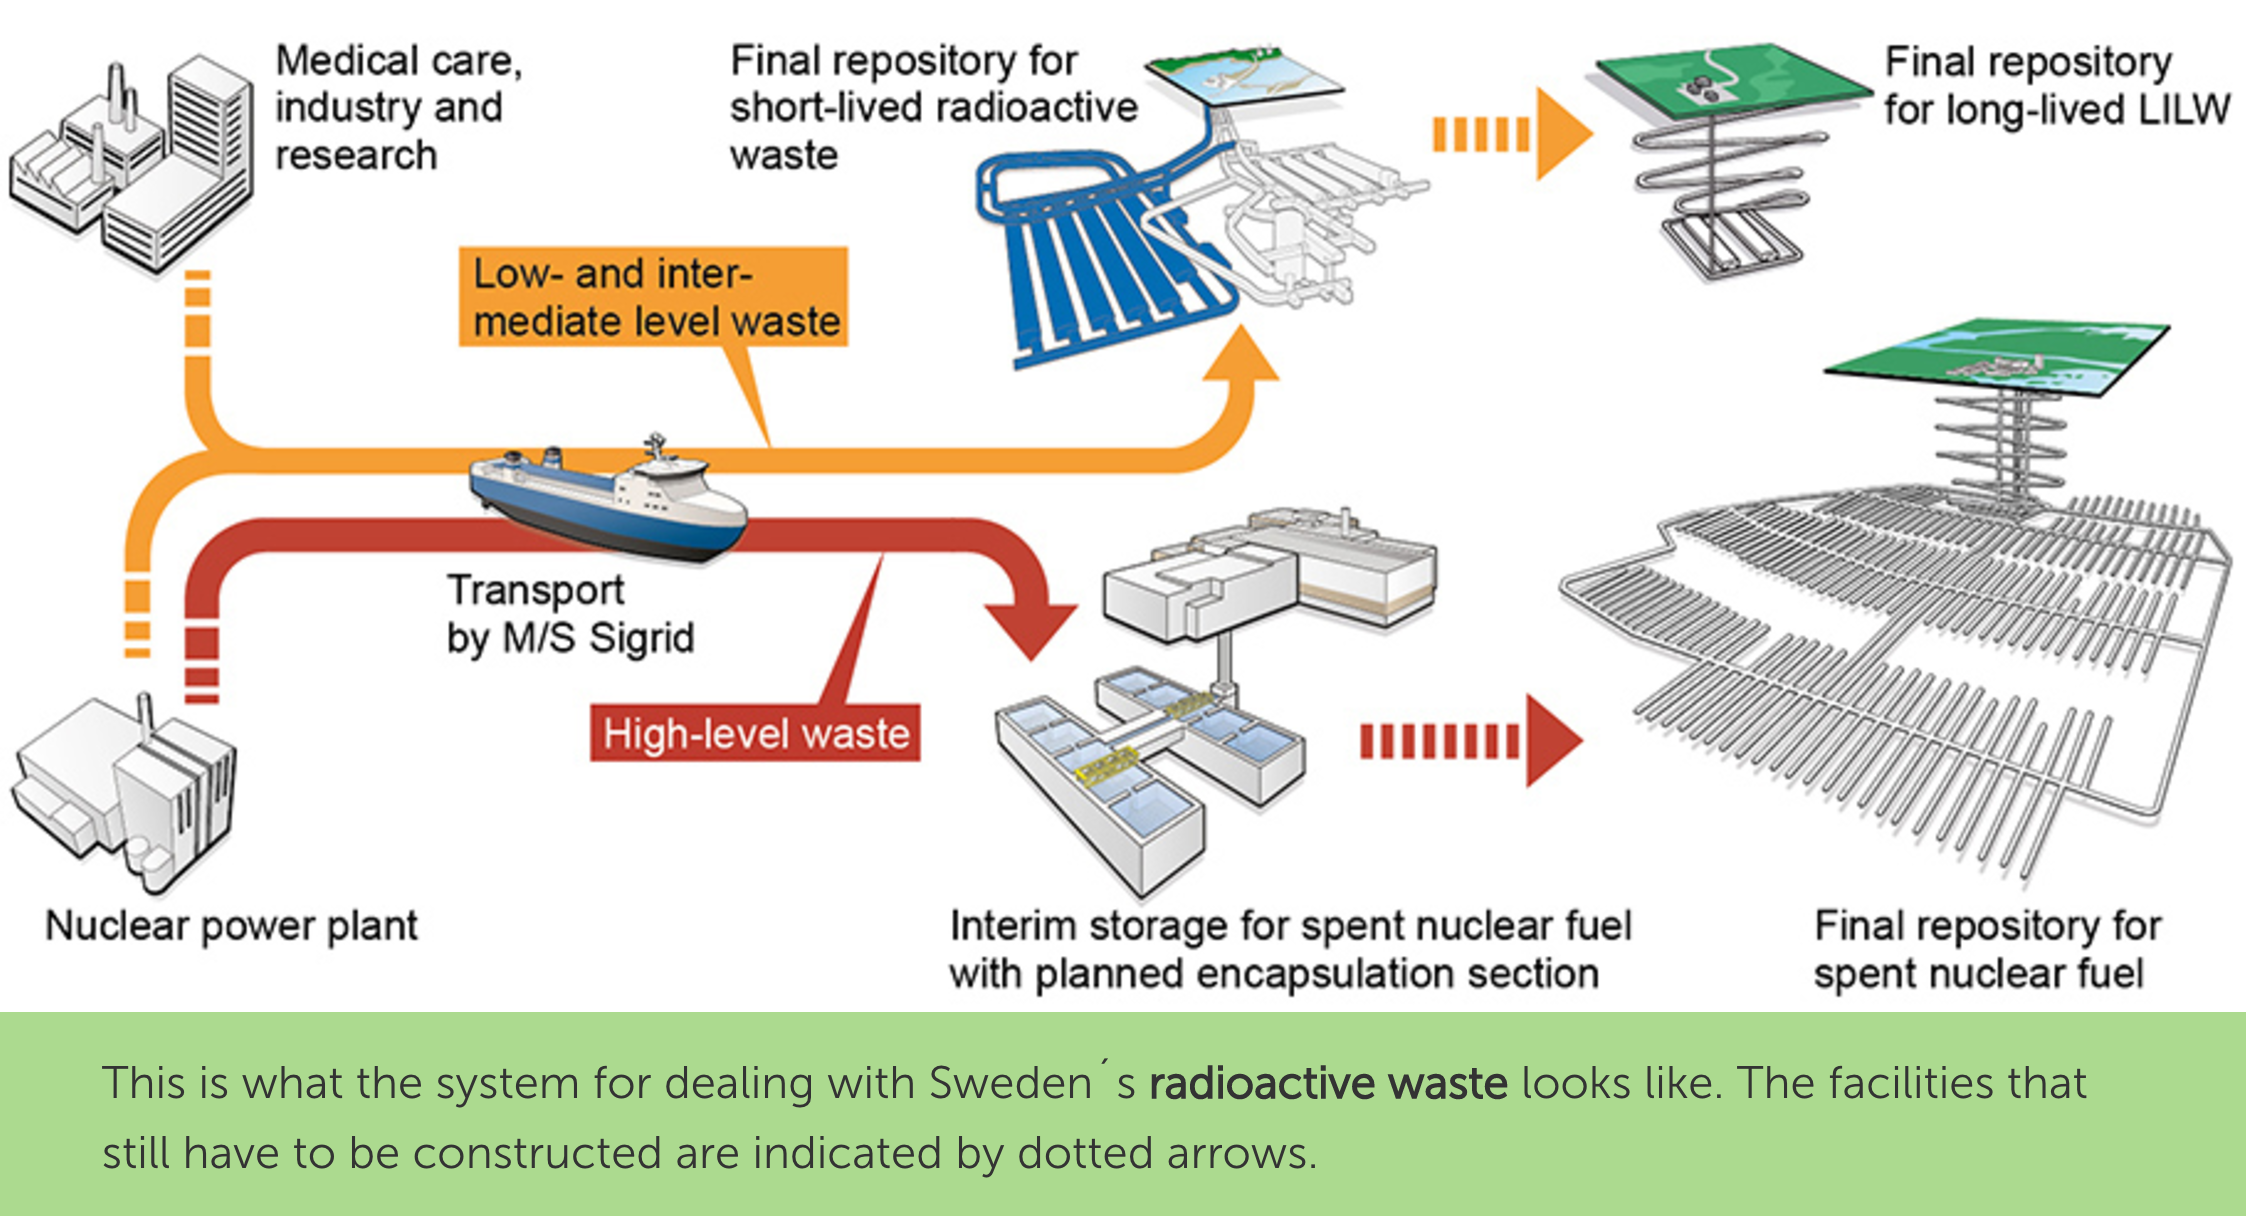
\includegraphics[width=\textwidth]{./images/sweden-plan}
\end{frame}


%%--------------------------------%%
\begin{frame}[c]
\frametitle{Sweden: Site}
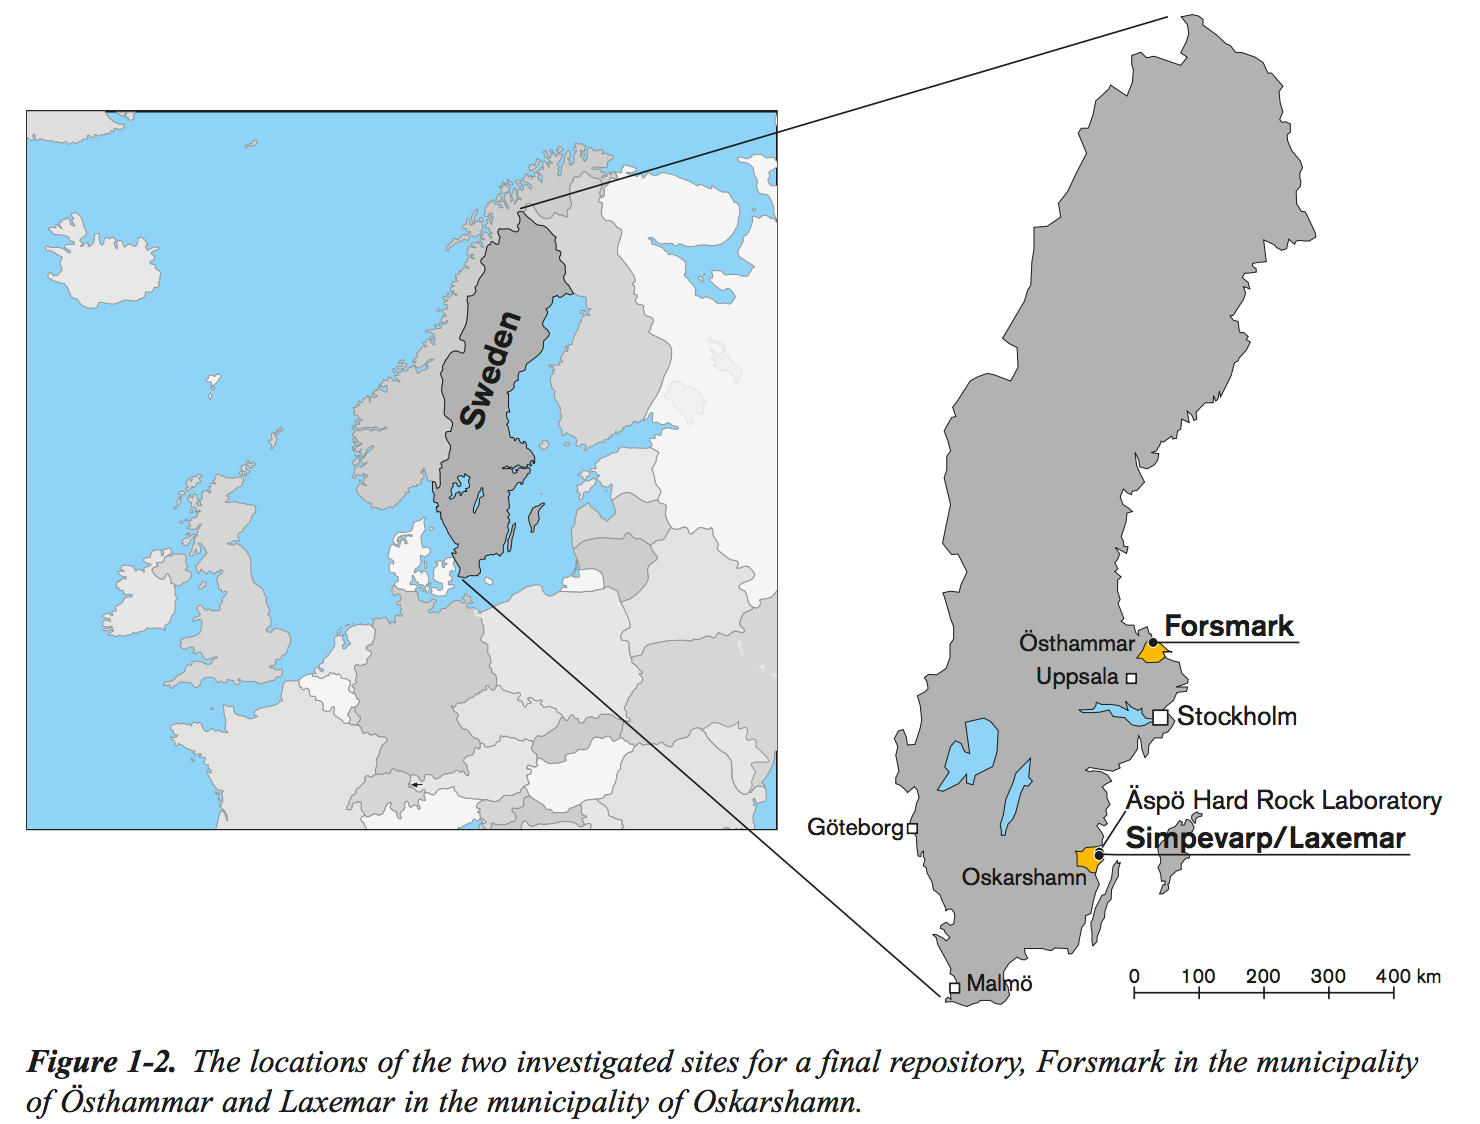
\includegraphics[width=\textwidth]{./images/sweden-site-selection}
\cite{skb_safety_2017}
\end{frame}

%%--------------------------------%%
\begin{frame}[c]
\frametitle{Sweden: Clab}

Clab - the Central Interim Storage Facility for Spent Nuclear Fuel is located at Simpevarp about 25 kilometres north of Oskarshamn. This is where all the spent nuclear fuel from Swedish nuclear power plants is kept while waiting for the final repository to begin operating.

\end{frame}


%%--------------------------------%%
%%--------------------------------%%
\begin{frame}[c]
\frametitle{Sweden: Short-Lived Radioactive Waste}
SKB’s Final Repository for Short-Lived Radioactive Waste is located
At Forsmark in the municipality of \"{O}sthammar. The facility started operating in 1988 and was then the first of its kind in the world.

\begin{itemize}
\item[\textbf{Operational start}] 1988
\item[\textbf{Capacity}] Approx. 63,000 cubic metres
\item[\textbf{Receiving capacity}] Approx. 600 cubic metres per year
\item[\textbf{Operational and maintenance staff}] Approx. 30
\item[\textbf{Above ground}] Offices and workshops, terminal building, ventilation plant
\item[\textbf{Underground}] Four rock vaults, one silo, control room
\item[\textbf{Operating costs}] Approx. SEK 40 million per year
\end{itemize}

The SFR is situated 50 metres below the bottom of the Baltic and comprises four 160-metre long rock vaults and a chamber in the bedrock with a 50-metre high concrete silo for the most radioactive waste. Two parallel kilometre-long access tunnels link the facility to the surface.
\end{frame}
%%--------------------------------%%
\begin{frame}[c]
\frametitle{Sweden: SKB}

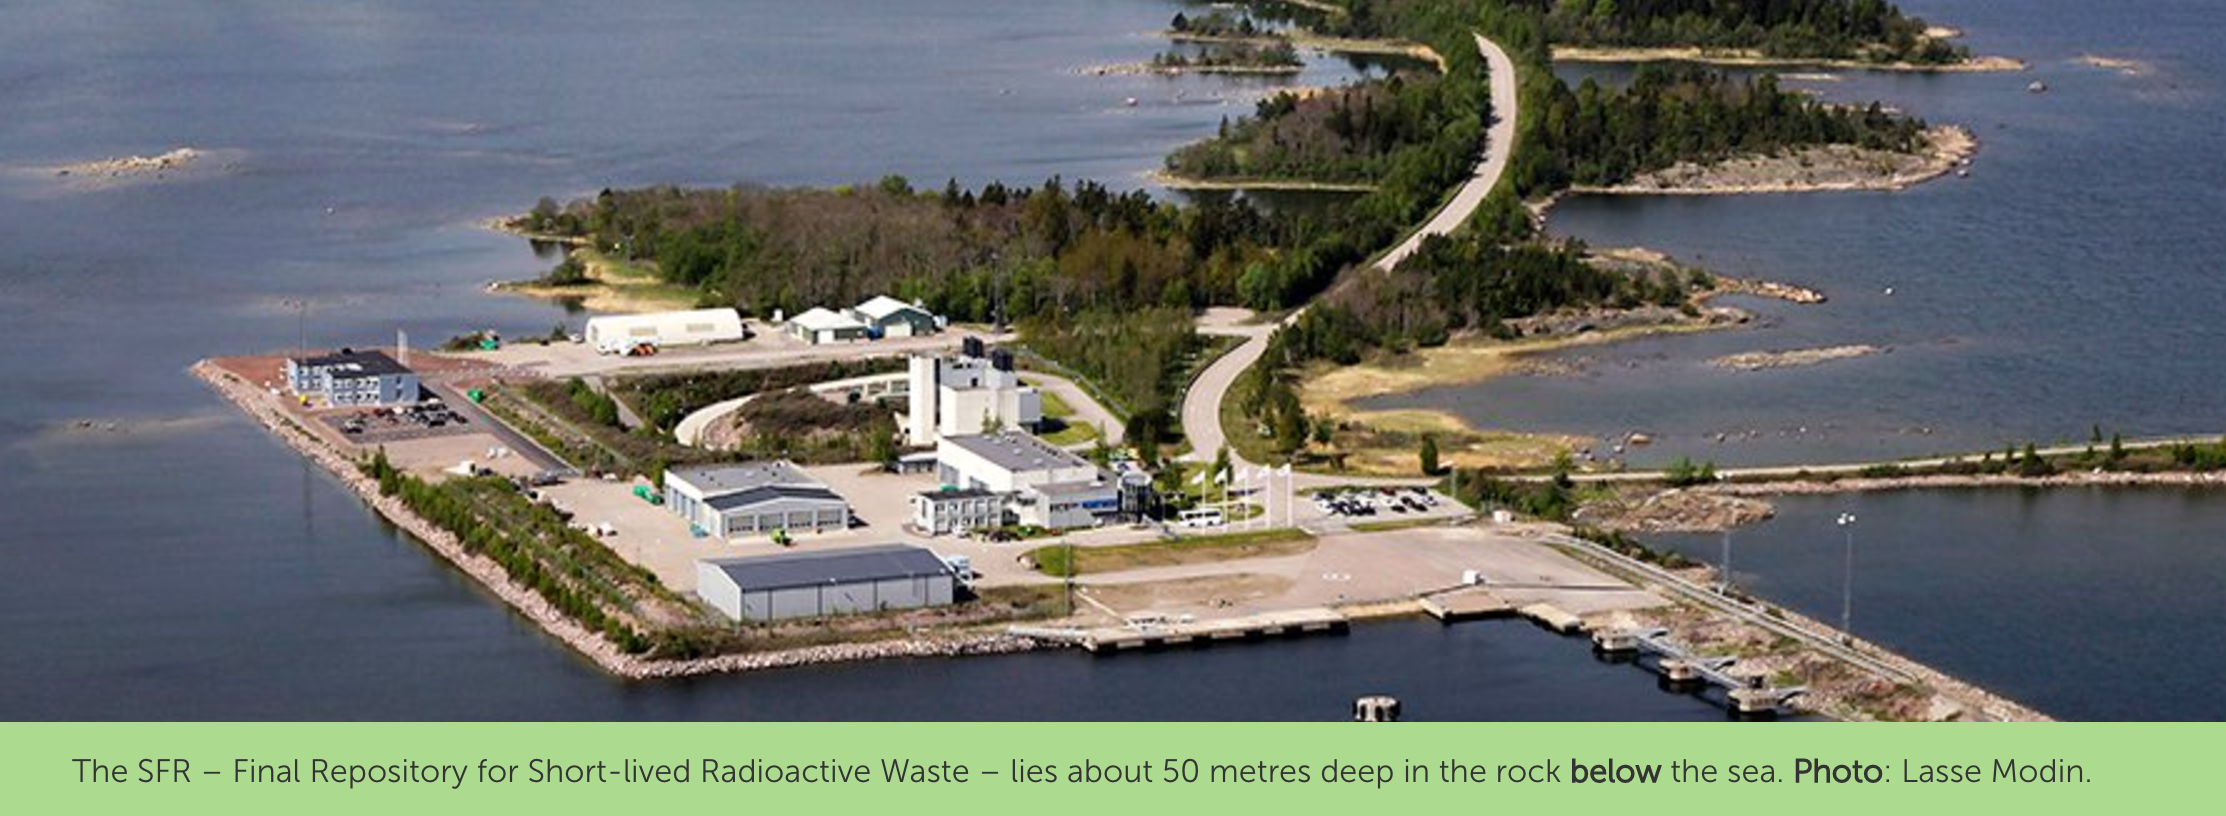
\includegraphics[height=\textheight]{./images/sweden-sfr}

\end{frame}

%%--------------------------------%%
%%--------------------------------%%
\begin{frame}[c]
\frametitle{Sweden: Final Disposal}

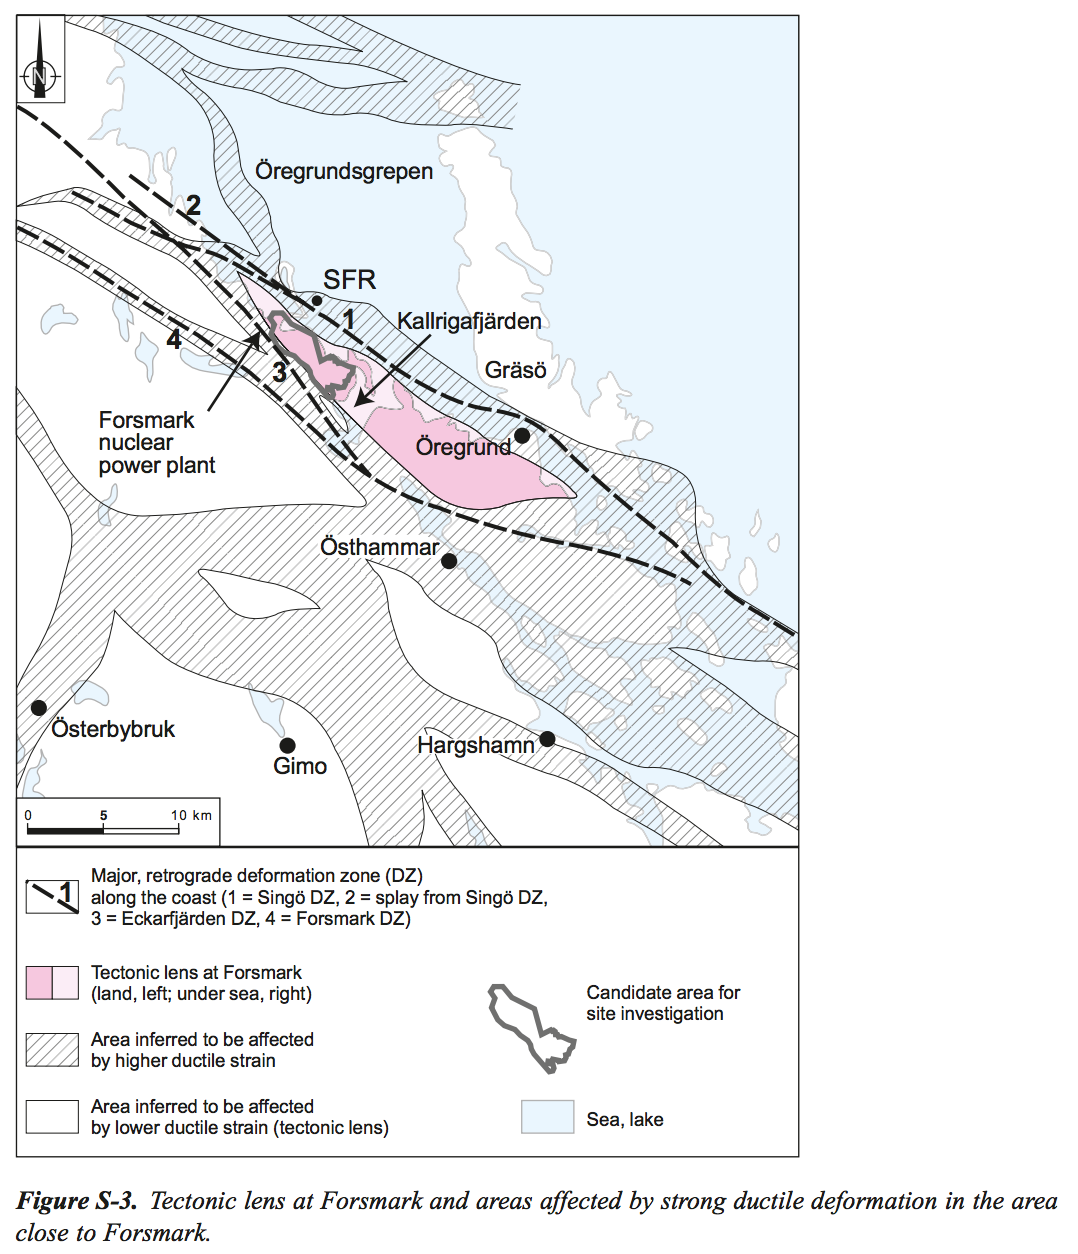
\includegraphics[width=\textwidth]{./images/sweden-forsmark-map}
From \cite{skb_long-term_2011}

\end{frame}
%%--------------------------------%%
\begin{frame}[c]
\frametitle{Sweden: Final Disposal}
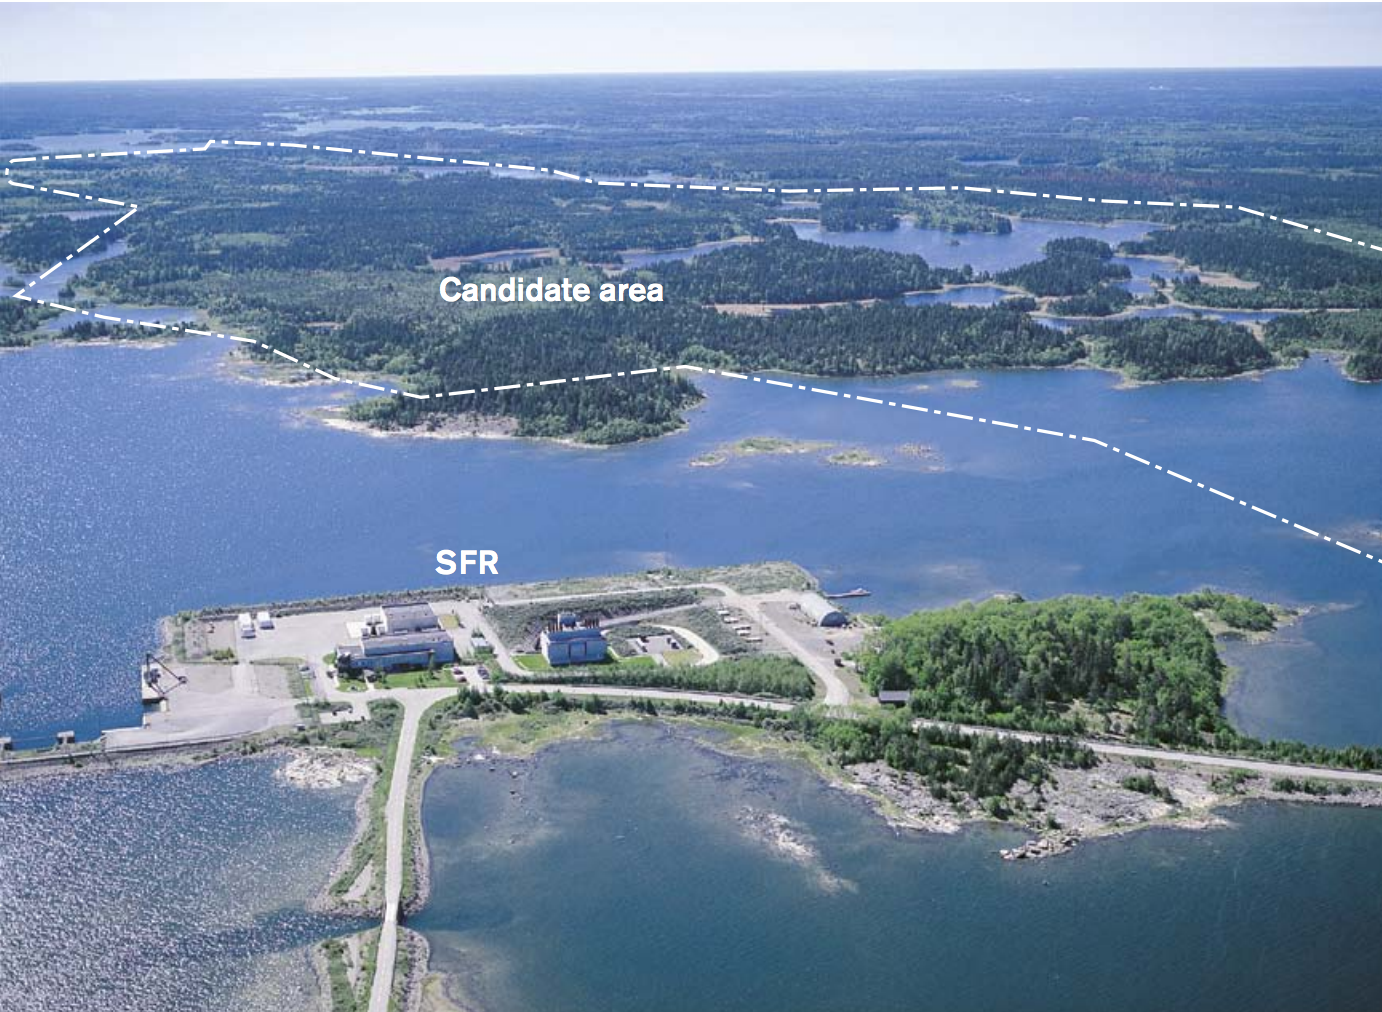
\includegraphics[width=\textwidth]{./images/sweden-forsmark-candidate}
From \cite{skb_long-term_2011}
\end{frame}

%%--------------------------------%%
\begin{frame}[c]
\frametitle{Sweden: Final Disposal}
sweden-forsmark-design.png
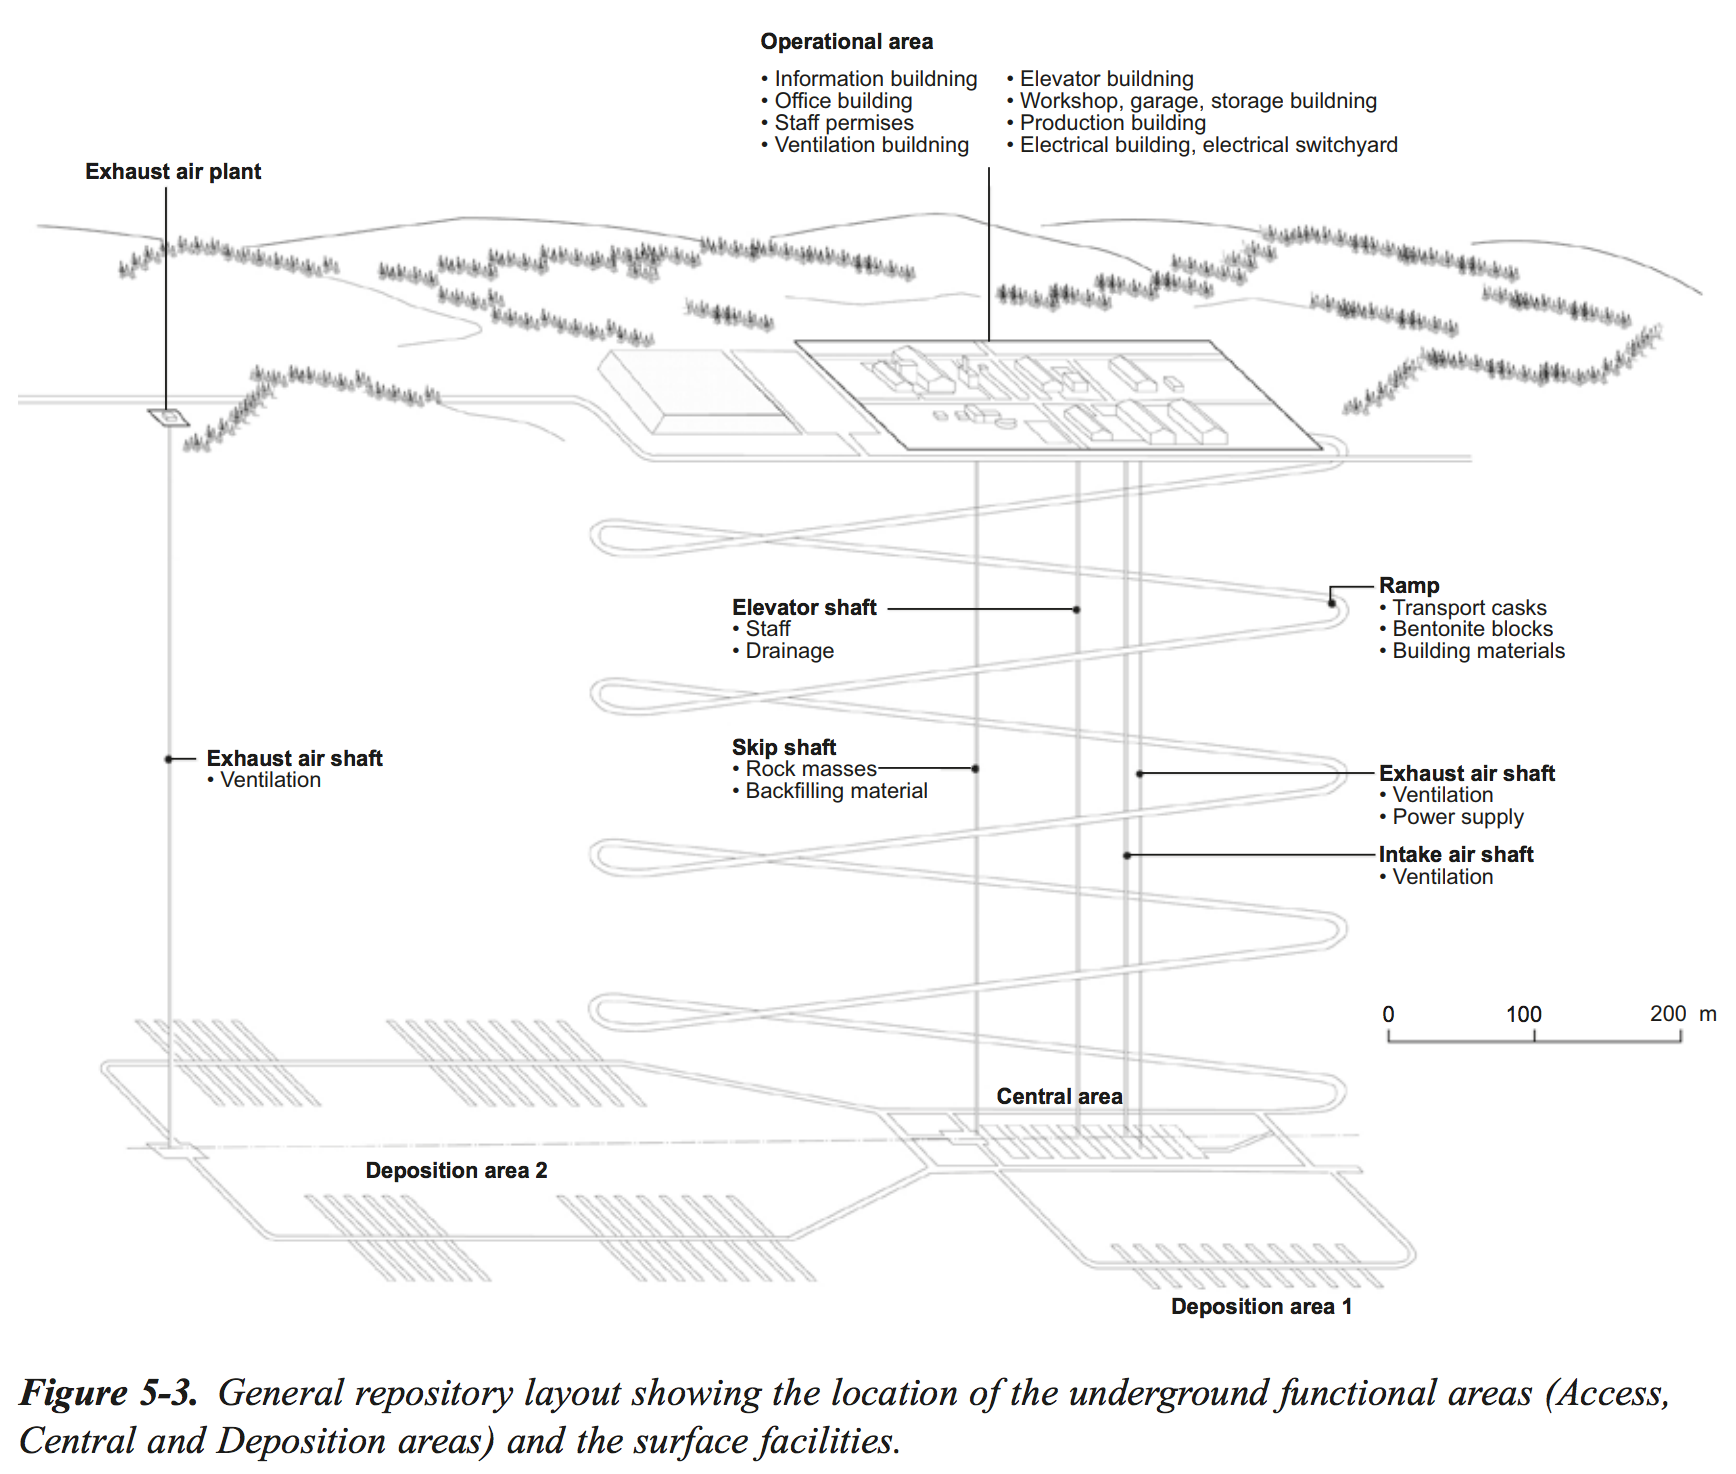
\includegraphics[width=\textwidth]{./images/sweden-forsmark-design}
From \cite{skb_long-term_2011}
\end{frame}

%%--------------------------------%%
\begin{frame}[c]
\frametitle{Sweden: Final Disposal}
sweden-forsmark-fractures.png
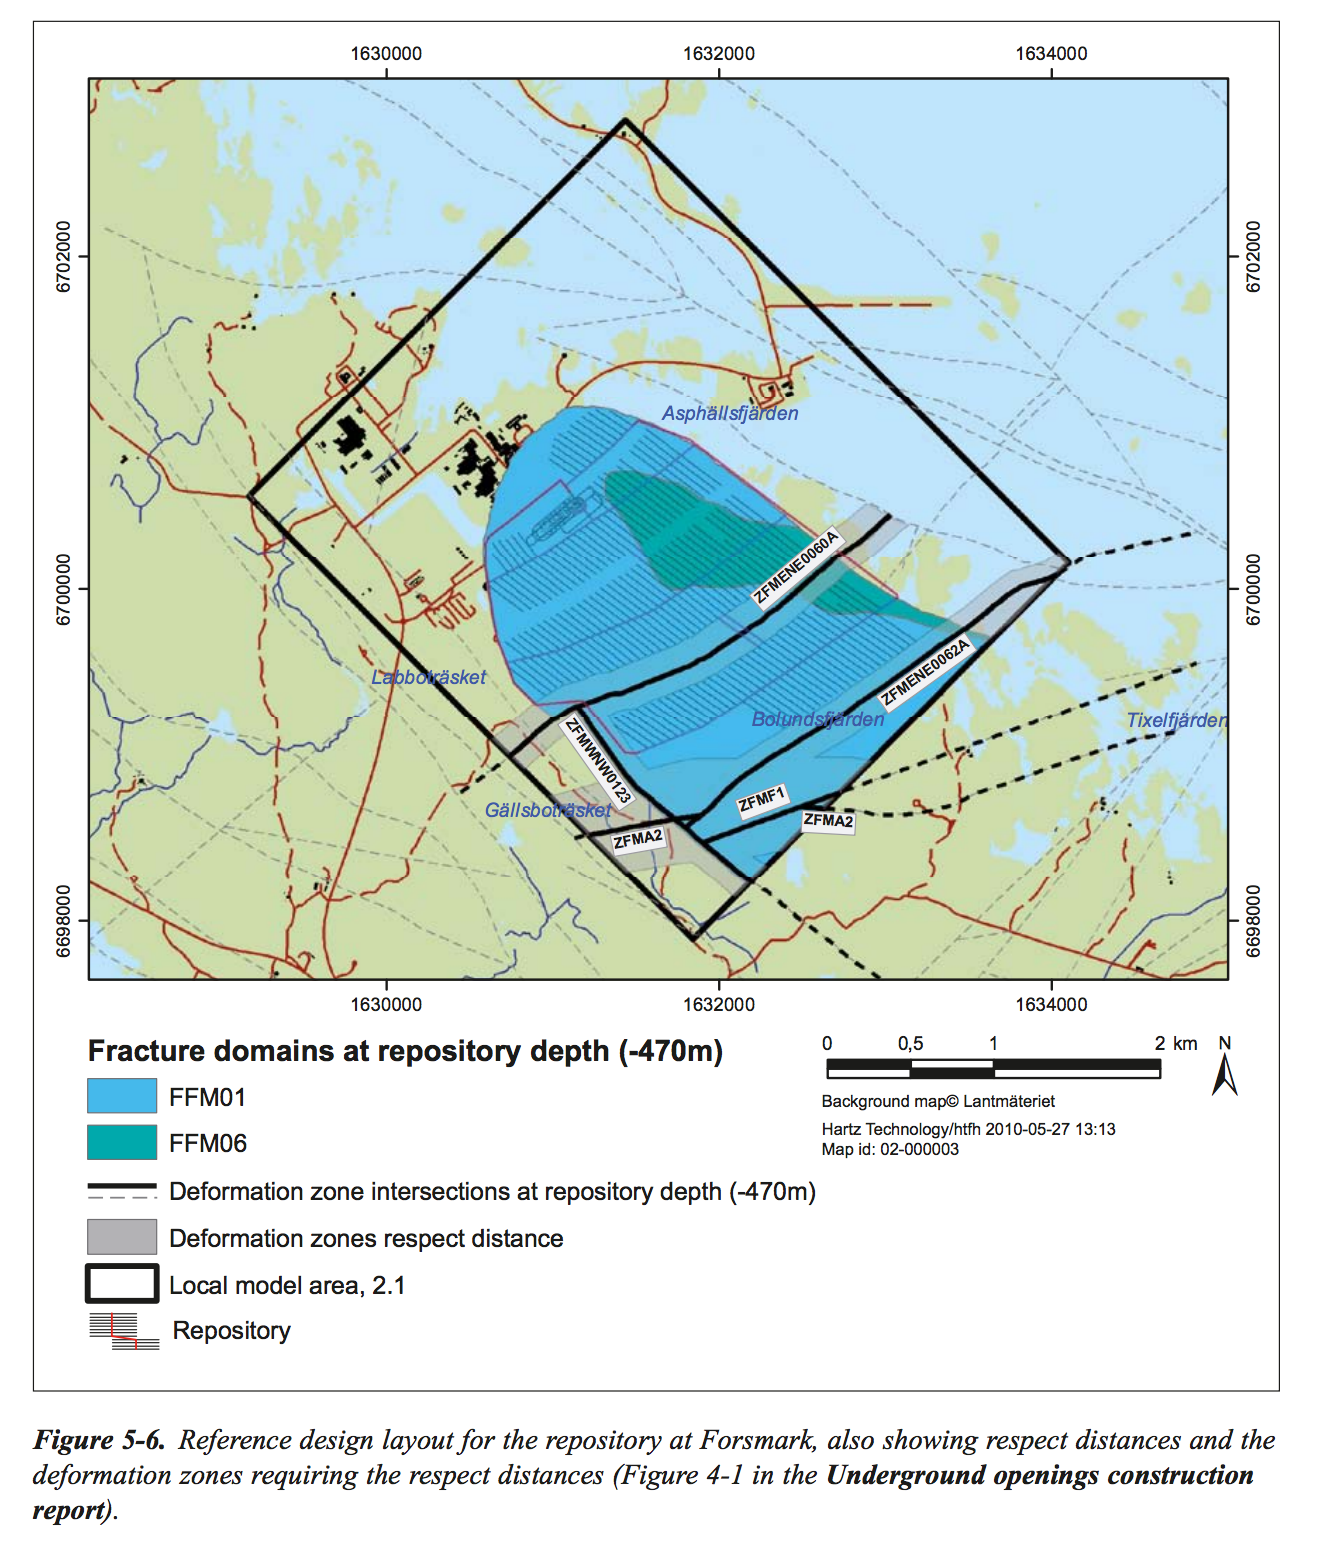
\includegraphics[width=\textwidth]{./images/sweden-forsmark-fractures}
From \cite{skb_long-term_2011}
\end{frame}


%%--------------------------------%%
\begin{frame}[c]
\frametitle{Sweden: Transport By Sea}

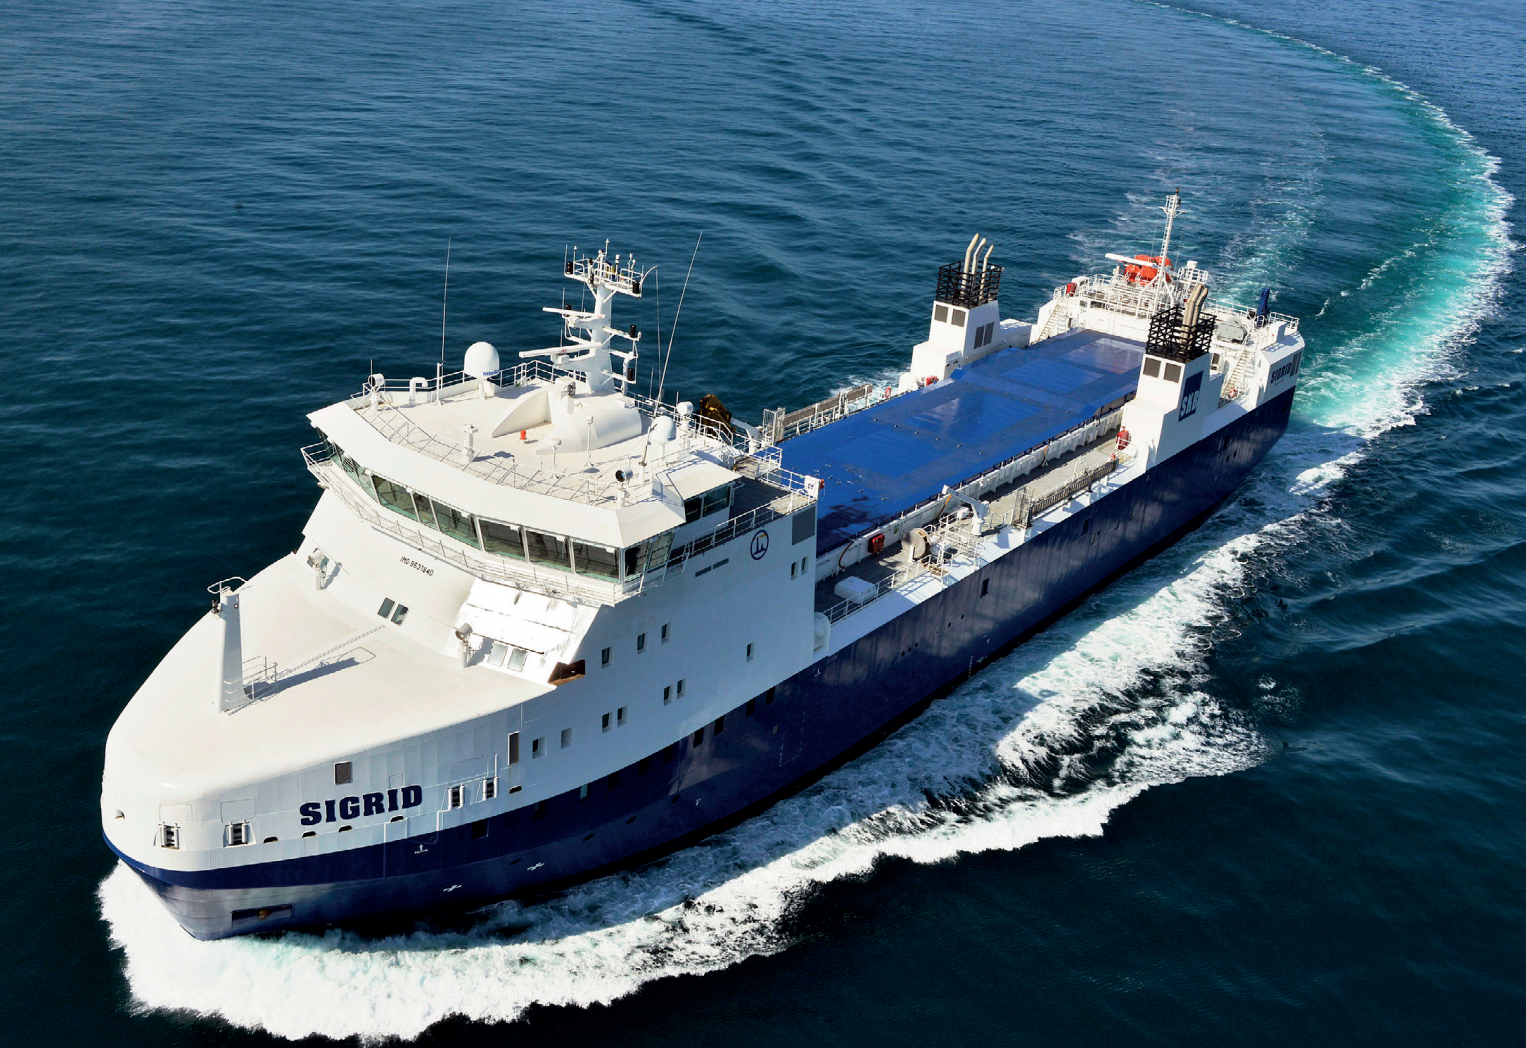
\includegraphics[width=\textwidth]{./images/sweden-sigrid}
Sigrid, the vessel which replaced Sigyn in 2013.

\end{frame}

%%--------------------------------%%
\begin{frame}[c]
\frametitle{Sweden: Transport By Sea}
\begin{center}
\begin{itemize}
\item[\textbf{Length overall}] 99.5 metres
                \item[\textbf{Primary cargo}] Radioactive waste and spent nuclear fuel
                \item[\textbf{Cargo capacity}] 12 transport casks or 40 freight containers
                \item[\textbf{Draught}] 4.5 metres
                \item[\textbf{Deadweight tonnage}] 1,600 tonnes
        \end{itemize}
\end{center}
\end{frame}
